% 第四章示例：说明结果写作，并展示脚注、公式、图表和程序代码。
\chapter{研究结果与规范表达}

\section{研究结果的组织}

研究结果部分应直接回应研究问题，并按照重要程度或分析逻辑组织
材料。作者需要先说明观察到的事实、数据或系统表现，再通过比较、
统计检验、案例证据或性能指标揭示其特征。正文不应逐项复述图表中的
全部数字，而应指出最值得关注的变化、差异、趋势和异常情况。

结果与讨论可以分章书写，也可以根据专业习惯合并。分章书写时，本章
主要呈现“发现了什么”，下一章重点解释“为什么出现这些结果”以及
“结果意味着什么”。无论采用哪种结构，都应区分客观结果与作者解释，
并确保每项结论都有相应证据支持。

\section{书写规范}

\subsection{使用语言}

原则上，毕业设计（论文）应采用国家语言文字工作委员会正式公布的
简化汉字书写。

\subsection{名词术语}

毕业设计（论文）中采用的术语、符号和代号必须全文统一，并符合相关
规范要求。

\subsubsection{科学技术名词}

科学技术名词应尽量采用全国科学技术名词审定委员会公布的规范词，
或国家相关标准中规定的名称。尚未统一规定或叫法有争议的名词术语，
可采用本学科惯用的名称。

\subsubsection{外文缩写和外国人名}

使用具有特定含义的术语、新名词或外文缩写时，首次出现应在圆括号
内注明含义或原文。外国人名一般可采用英文原名，广为人知的人名可按
通行标准译法书写。

\subsubsection{计量单位}

计量单位应符合国家标准 GB 3100～3102—93。非物理量的单位，如件、
台、人和元等，可使用汉字与符号构成组合单位，例如件/台、元/km。
单位名称应全文统一，不应混用中英文名称。

\subsection{数字和标点符号}

标点符号应符合《标点符号用法》（GB/T 15834—2011）。涉及测量和
统计的数据一般使用阿拉伯数字，在普通叙述中则应根据语言习惯合理
选择数字形式。

\section{注释与公式}

\subsection{注释}

正文中有个别名词或情况需要解释时，可以采用脚注。脚注序号以页为
单位，每页从 1 开始编号，正文中的编号使用上标；注释应置于注释
符号出现的同一页，不得隔页。\footnote{脚注可用于补充不宜在正文
展开、但有助于读者理解的说明。}

\subsection{公式}

数学公式用于准确表达变量之间的关系，重要公式应在正文中加以解释
和引用。二项式展开可写为
% equation 会自动按章编号；label 用于正文中的交叉引用。
\begin{equation}
  (1+x)^n
  = 1 + \frac{nx}{1!}
  + \frac{n(n-1)x^2}{2!} + \cdots .
  \label{eq:binomial}
\end{equation}

傅里叶级数可表示为
\begin{equation}
  f(x)=a_0+\sum_{n=1}^{\infty}
  \left(a_n\cos\frac{n\pi x}{L}
  +b_n\sin\frac{n\pi x}{L}\right).
  \label{eq:fourier}
\end{equation}

长公式不能在一行排完时，原则上应在等号或运算符处换行，并使运算符
位于续行行首。需要解释变量时，可在公式后使用“式中：$a_n$ 为余弦
项系数，$b_n$ 为正弦项系数”的形式说明。

\section{图表表达}

图表标题应简洁、精炼并具有自明性。图表应在正文首次提及之后给出，
并与相邻文字形成清晰、连贯的论证关系。

\subsection{图}

插图应保持背景清晰，横纵坐标的变量名、单位和刻度应完整。
图~\ref{fig:distribution} 给出了统计分布示例。

% 插图：先在正文中提及，再放置 figure；caption 在 label 之前。
\begin{figure}[htbp]
  \centering
  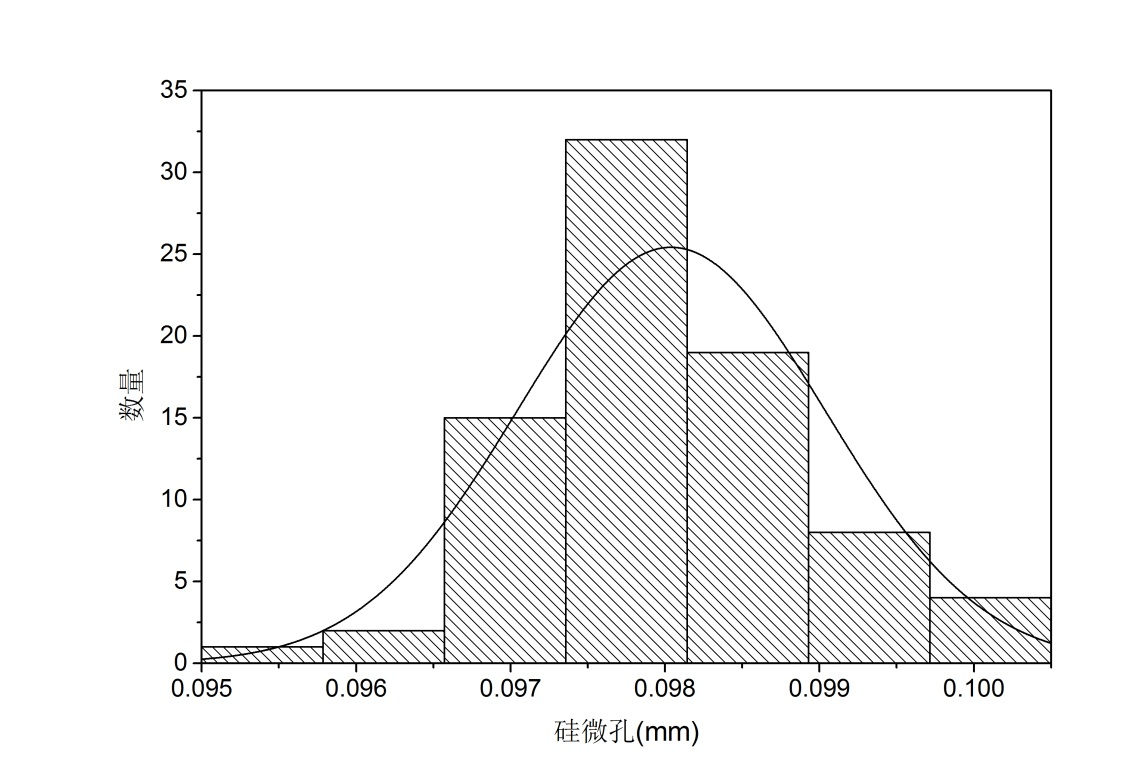
\includegraphics[width=0.72\textwidth]{assets/word-figure-3-1.jpeg}
  \caption{9×9 阵列硅微孔直径统计分布图}
  \label{fig:distribution}
\end{figure}

多幅相关图像可以组合为一幅分图，并以（a）、（b）、（c）等标出，
便于在正文中分别讨论和相互比较。

% 组合图：两个 minipage 分别承载一个分图。
\begin{figure}[htbp]
  \centering
  \begin{minipage}[t]{0.46\textwidth}
    \centering
    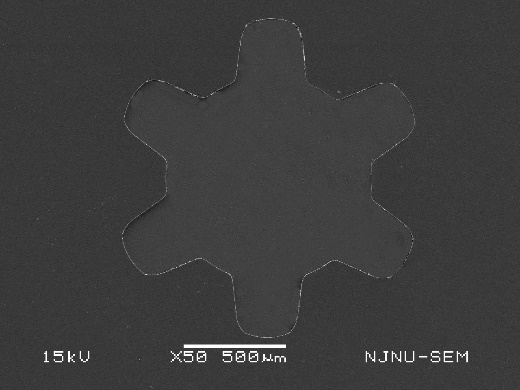
\includegraphics[width=\linewidth]{assets/word-figure-3-2a.jpeg}\\
    （a）单联硅齿轮
  \end{minipage}\hfill
  \begin{minipage}[t]{0.46\textwidth}
    \centering
    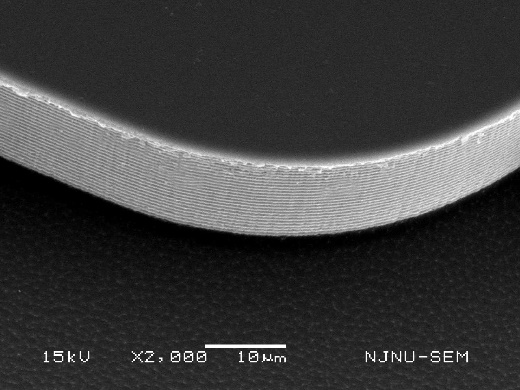
\includegraphics[width=\linewidth]{assets/word-figure-3-2b.jpeg}\\
    （b）硅齿轮局部
  \end{minipage}
  \caption{ICP 刻蚀的硅微齿轮模具 SEM 照片}
  \label{fig:sem}
\end{figure}

\subsection{表}

表格适合呈现具有共同字段、便于横向比较的数据。表头应准确概括
各列含义，数值精度和计量单位应保持一致。

% 表格：caption 和 label 写在表体之前。
\begin{table}[htbp]
  \centering
  \caption{单个硅齿轮（$z=6$）测量尺寸}
  \label{tab:gear}
  \begin{swuttable}
    \begin{tabular}{ccc}
      \toprule
      齿顶圆直径 $d_a$/mm & 齿根圆直径 $d_f$/mm
        & 同轴度误差/mm \\
      \midrule
      1.5530 & 0.9979 & 0.0129 \\
      1.5465 & 1.0003 & 0.0042 \\
      1.5571 & 0.9985 & 0.0045 \\
      1.5471 & 1.0000 & 0.0045 \\
      1.5539 & 0.9987 & 0.0098 \\
      1.5472 & 1.0004 & 0.0052 \\
      \bottomrule
    \end{tabular}
  \end{swuttable}
\end{table}

\begin{table}[htbp]
  \centering
  \caption{产品统计表}
  \label{tab:statistics}
  \begin{swuttable}
    \begin{tabular}{lrrrr}
      \toprule
      产品 & 产量 & 销量 & 产值 & 比重 \\
      \midrule
      手机   & 11000 & 10000 & 500  & 50\% \\
      电视机 &  5500 &  5000 & 220  & 22\% \\
      计算机 &  1100 &  1000 & 280  & 28\% \\
      \midrule
      合计   & 17600 & 16000 & 1000 & 100\% \\
      \bottomrule
    \end{tabular}
  \end{swuttable}
\end{table}

\section{伪代码和程序代码}

程序代码可用于说明研究中的核心算法、数据处理流程或关键实现。
以下代码给出了一个简短的控制台程序示例。

% 代码块会在空间不足时整体换页，并保持与后文的源文件顺序。
\begin{lstlisting}[language={[Sharp]C}]
using System;

namespace ConsoleApp1
{
    class Program
    {
        static void Main(string[] args)
        {
            Console.WriteLine("Hello World!");
        }
    }
}
\end{lstlisting}
